% GENERATED FROM typst/manual/sections/00_native_closure_wave_temporal_fixtures.typ BY scripts/typ2tex.py (v1.0.0) — DO NOT EDIT.
% Edit canonical Typst under typst/ and regenerate with: python3 scripts/typ2tex.py --root . --outdir latex

\section{Native closure, wave and temporal fixtures}\label{manual:m1-native-fixtures}

\paragraph{Calculation card.}
Native certificates, scopes and committed prefixes are exact fixture inputs.
The runner below computes closure, recurrence, directional contact and flux
outputs against exact comparators; its hostile controls are the falsifiers.
Only the final demonstration uses a declared rational report calibration.
Physical input uncertainty is uninstantiated. The common method is
\secref{manual:calculation-spine}.

The executable motif and fold fixtures use a declared preassembled-prefix
realization: component closures complete before the target trace starts.
This is a sufficient causal realization of the Main's more general
commit-before-consumption rule. Each outer trace binds its inner identity,
certificate set and scope map before certification. A further distinct outer
return supplies the outer beat; exposure preserves the bound inner wave.
Duon fixtures separately execute the twelve support signatures, carried current,
distinct recurrent returns and the Duad's seated state of the same identity
(\mainequation{main:eq:duad-same-current}).
The finite harmonic readout declares a cyclic index group and committed window;
every recorded state contains only the certificate, cadence and phase prefix
available at that return. Its projection is a declared model record.
In the executable compatibility record, \texttt{edges} counts phase-bearing
atomic traversals and \texttt{phases} counts complete certified closure-phase
cycles. Thus the minimal two-edge return has $(2,1)$, while the four-edge
return has $(4,1)$. The legacy key \texttt{phases} is retained to avoid an
engine-schema break; it never counts edges, dwell, or Fourier coefficient phase.

\paragraph{Record class and execution.}
These are native exact witnesses or explicitly declared models. The shared
runner is \texttt{manual/scripts/aod\_native\_closure\_wave.py}; its five CSV
inputs preserve trace, scope, lineage, expected exact result and hostile case.
The command \texttt{python3 manual/scripts/aod\_native\_closure\_wave.py --check-data}
executes the rows. An expected rejection is a successful hostile check only
when the actual law rejects the supplied input. Actual results are recorded
separately from these immutable inputs.

{\footnotesize
\begin{longtable}{>{\raggedright\arraybackslash}p{0.230\linewidth}>{\raggedright\arraybackslash}p{0.330\linewidth}>{\raggedright\arraybackslash}p{0.340\linewidth}}
\toprule
Construction & Exact witness & Hostile control \\
\midrule
\endfirsthead
\toprule
Construction & Exact witness & Hostile control \\
\midrule
\endhead
Null/anchor & Five distinct types; first $00_8$ & Prior coordinate choice or type collapse \\
Atomic support & H1 legs, composite H2 and closed H0 endpoints & Direct H2 called atomic \\
Hinge/cycle & $\varepsilon0_H(0_D)^m(-\varepsilon)$, $m=0,2$, one closure-phase cycle & Bypass, same-sign end, replay recount \\
Reflected legs & $1+1=2$, $1+3=4$ phase-bearing steps; unit embedding $1_C\mapsto2h$ & One-step trace; unequal-leg factorization; support bound without closure witness \\
Recurrence & Three bound closures give two beats, separations $(10,10)$ & One closure or repeated certificate \\
Kernel & Weights $(1,1)$ or $(1,3)$ on admitted support & Bypass mass; empty normalization \\
Motifs & Dion, two-Monon Dimonon, 12 Duon variants, Duad state & Collapsed names or changed certificate bytes \\
Fold/exposure & One outer closure-phase cycle, retained inner wave & Contact called closure; lower beats reused \\
Temporal pair & Ratio, bias, unwrapped lag, directional RCD & Aliases, one contact, zero denominator \\
State/update & Equal temporal view, different pressure; later response & Future input or projection/state collapse \\
Flux/Stokes & AFC $0$ or $1/2$; AOD $7$, boundary $3$ & Pressure in normalized memory; wrong reverse sign \\
FRG & Independent $5$, cross $3$, recurrent $8$ & Model before admission; same-step response \\
Harmonics & $(1,0,-1,0)$ reconstructs exactly & Unbound word gains admission \\
Conservation & Active closure-phase-cycle equation binding & Mapping that source to an unrelated Fourier equation \\
Report & $Nn=3(2/3)=2$, $4(2/3)=8/3$ & Missing calibration; $3n$ used for $N=4$ \\
\bottomrule
\end{longtable}
}

\paragraph{Reflected-leg and flux controls.}
An asymmetric certified $1+3$ return has four phase-bearing steps and one
closure-phase cycle. Its total $4h$ equals neither doubled leg, $2h$ nor
$6h$, although both doubled legs satisfy the reference lower bound.
For the AFC two-state swap kernel, memory $(3/4,1/4)$ gives flux $1/2$;
equal memory gives zero. Under exchange of the two states, the unequal-memory
flux reverses sign even though the kernel is unchanged. These controls use
\mainequation{main:eq:reflected-leg-bound} and \mainequation{main:eq:flux-types}.

\paragraph{Field-count calculation.}
One admitted recurrent monon-mode wave organization has $n_F=1$ and
$\mathcal{O}_{\partial F}=0$ under \mainequation{main:eq:field-count-term}.
Alias names do not create another field; an isolated monon supplies no field.

\paragraph{Disoma declaration.}\label{subsec:disoma-declaration}
For a two-field declared scope, fix

\[
B_{12}=(\partial F_{12},\omega_{12}),\qquad\mathcal{F}_{B_{12}}=\{F_1,F_2\}.
\]

Thus

\[
n_F(B_{12})=2,\qquad\mathcal{O}_{\partial F}(B_{12})=2\log2.
\]

\begin{figure}[H]
\centering
\fbox{\begin{minipage}{0.88\linewidth}\centering
Scope $\mathcal{B}=(\partial F,\omega)$ and resolved organizations
$\mathcal{F}_{\mathcal{B}}=\{F_1,\dots,F_{n_F}\}$ 

$n_F=|\mathcal{F}_{\mathcal{B}}|$, declared count term $n_F\log n_F$ 

A single recurrent monon-mode wave organization has $n_F=1$. 

A lone monon closure supplies one complete closure-phase cycle; field membership requires recurrence.
\end{minipage}}
\caption{Fixed-scope field count and SADAR scope.}
\label{fig:field-count}
\end{figure}

\paragraph{Prefix validation and scalar storage.}
Each construction record stores its exact prefix digest and witness. Validation
checks those bindings against the declared registry, including the closure,
return, motif and both contact prefixes of
\mainequation{main:eq:closure-certificate},
\mainequation{main:eq:return-identity}, \mainequation{main:eq:motif-admission}
and \mainequation{main:eq:coupling-trace}. Unknown, empty or mismatched records
reject before model or harmonic use. A registry or reconstructed cache validates
an existing construction; it cannot originate distinction or recurrence.
An implementation declares its update law and admissible input domain before
executing \mainequation{main:eq:wave-update-trace}. The additive duration
implementation stores $(RD,r_1,\dots,r_m)$, with $r_s\ge0$, then applies
\mainequation{main:eq:rcd-additive-realization}; reversal recomputes the
reflection counts. A polyrhythm calculation follows cycle provenance first,
then stores scalar A$\Omega$ accessors. A raw duration cannot replace the
branch/hinge/branch data needed by later coupling, seat compatibility or shedding.
The scalar outputs are derived caches of their bound constructions.

\paragraph{Periodic support calculation.}
Use \mainequation{main:eq:fractal-tesseract-cycle-range} and the single-hinge
support formulas of \mainappendix{main:app:rd-tests:corollaries}.
For $3:4::3:3::6$, the support types are

\[
C_{\sigma}[3:4;C_6]_{\AO},\qquad C_{\sigma}[3:3;C_6]_{\AO},
\]

with $|\Sigma_{\mathrm{support}}|=2$. In the declared symmetric single-hinge, neutral-reflection periodic specialization, choose recurrence periods equal to these RD accessors; then

\[
RD_{\AO}(3:4)=137,\qquad RD_{\AO}(3:3)=61,\qquad T_{\mathrm{sync}}=\operatorname{lcm}(137,61)=8357.
\]

The coupling is $\SADARop_B(C_{3:4},C_{3:3})$. Adjacency and the
least common multiple alone do not establish that coupling.

\begin{figure}[H]
\centering
\fbox{\begin{minipage}{0.92\linewidth}\centering
\textbf{Fractal-tesseract support family} 

$\mathfrak{a}$ fractal range $+$ section grade $r$ $+$ $\Sigma=(3:4,3:3;C_6)$ 

$\downarrow$ 

$\operatorname{cycle}\langle\mathfrak{a},r\rangle(\Sigma)$ 

$\downarrow$ 

$C_{\sigma}[3:4;C_6]_{\AO}$, $C_{\sigma}[3:3;C_6]_{\AO}$ 

$\downarrow$ 

tesseract sections count support occurrences; $\SADARop_B$ couples beats
\end{minipage}}
\caption{Fractal-tesseract cycle range and support family.}
\label{fig:fractal-tesseract-beat-family}
\end{figure}

\paragraph{Directional count realization.}
Both wave identities and repeated contact-prefix digests are bound before
comparison. With support $RD=3$ and two reflection counts, the declared
additive interface gives $\rho^D_{a|b}=3+1+1=5$ and
$\rho^D_{b|a}=3+2+2=7$. The ratio reverses reciprocally, signed offsets
reverse, and the directional duration is recomputed. A same-domain window of
two clips only participation to two; it changes neither RD nor RCD.
The native count comparator has $\Lambda=N_a-N_b+b_a-b_b$, with drift
formed against the preceding committed comparison. A whole-closure slip
changes this unwrapped value even when a separately wrapped display repeats.

\paragraph{Interface composition.}
A recurrent $8\to9\to8$ realization initializes at vertex 8 and composes
with the committed-return readout. Primitive Duon components and targets share
their resolution; cross-scale composition uses the explicit folding map.
The comparison takes precisely two rational offsets; contact commitments,
window endpoints and update cuts are integers. Contacts use closed window
support $[u,v]$, while return counts use $(u,v]$. A lineage retains its ancestor identity
under a fixed coordinate relabelling; a substituted ancestor is rejected.
Every outer certificate carries the admitted inner waves and their bound
scope map. The controls reject missing fold provenance, unrelated-scale
pivots, malformed windows and fractional cuts, preserving rational currents.
These controls run with \texttt{python3 -m pytest -q}
\texttt{tests/test\_native\_closure\_wave.py}.

\paragraph{Calibrated report boundary.}
The emitter/mirror record uses $N=\Delta\mathrm{bip}_{\mathrm{return}}$ and
$x^{\mathrm{mir}}=Nn$. The displayed $x=3n$ is restricted to $N=3$.
A metrology record declares measurand, protocol, reference realization,
coupling/probe, detector, calibration, unit, resolution, uncertainty,
repeatability and traceability. The rational multiplier in this demonstration
is a declared report calibration, not an empirical calibration or native time unit.

\subsection{Wavelet continuation, recipient stages and harmonic scope}\label{manual:wavelet-continuation-fixtures}

\paragraph{Setup.}
A localized wavelet continuation (\mainsection{main:subsec:aod-wavelet-continuation},
\mainequation{main:eq:aod-wavelet-continuation}) restricts an admitted parent
current $W_{\mathrm{parent}}$ to a declared boundary/window
$B=(\partial F,\omega)$ with ordered integer cuts $\omega=(u,v]$, retaining
its parent identity, ancestry, support, window, committed prefix records and
return witnesses without terminating $W_{\mathrm{parent}}$ beyond $v$.
Its seating coordinate $\sigma_{\mathrm{seat}}\in\{\mathrm{open\_duon},\mathrm{seated\_duad}\}$ (\mainequation{main:eq:duad-same-current}) and
coupling/route role $\sigma_{\mathrm{role}}\in\{\mathrm{local\_segment},\mathrm{coupled\_segment},\mathrm{shed\_continuation}\}$ vary independently:
a seated Duad retains its open-Duon identity and structural $0_H$ hinge,
may remain a $\mathrm{coupled\_segment}$, and does not lose retained seating
when emitted as a $\mathrm{shed\_continuation}$.

\paragraph{Derivation.}
Fix a parent lineage $W_{B,1}$ on scope $B$ with initial origin closure
$C_0$ at cut $0$ ($j=0$) and compatible returns $C_1,C_2,C_3$ at cuts
$2,6,8$ ($j=1,2,3$), bound to an injective canonical occurrence registry
(derived from \texttt{Trace.return\_id} and admitted certificates when native
traces are supplied, or validated as declared finite-model occurrences with
display labels kept separate from immutable occurrence payloads). Under
\mainequation{main:eq:wavelet-overlap-dedup}:

\begin{itemize}
\item \emph{Retained support versus eligible in-window returns.} On
$\omega=(3,5]$, retaining prefix witnesses $(C_0@0,C_1@2)$ preserves full
support while contributing $R_1((3,5])=\emptyset$ and $q_1((3,5])=0$. On
$\omega=(-1,1]$, containing only the initial origin $C_0@0$ contributes
$1$ closure-phase cycle and $0$ reclosure beats. On half-open $(2,6]$,
the left endpoint $C_1@2$ is excluded and the right endpoint $C_2@6$ is
included, giving $R_1((2,6])=\{C_2\}$. Same-scope witnesses apply directly;
distinct scopes require an explicit identity-preserving scope map rather than a
default flag.
\item \emph{Overlapping complete windows.} The complete windows
$\omega_1=(0,6]$ ($R_1(\omega_1)=\{C_1,C_2\}$, $q_1=2$) and
$\omega_2=(4,8]$ ($R_1(\omega_2)=\{C_2,C_3\}$, $q_1=2$) share
$C_2@6$. Their per-window sum is $2+2=4$, whereas immutable
$\operatorname{id}_{\mathrm{return}}$ union deduplication gives
$q_1(\omega_1\cup\omega_2)=\#\{C_1,C_2,C_3\}=3$.
\item \emph{Shed continuation and recipient stages.} Under
\mainequation{main:eq:shed-continuation-witness} and
\mainequation{main:eq:recipient-event-lattice}, routed surplus $w_{\mathrm{shed}}$
retains parent identity, emission boundary, cut coordinate, emission cut, route
tag, routed amount and post-shed parent state. At recipient scope
$B_{\mathrm{rec}}$, delivery, acceptance and seating require their own
witnessed stage events ordered consistently with emission on the declared cut
coordinate (or an explicit coordinate relation); the passive branches
$\mathrm{emitted}\to\mathrm{delivered}\to\mathrm{unaccepted\_pass}$,
$\mathrm{accepted}\to\mathrm{pending\_unseated}$, and $\mathrm{seated}$
each contribute $\Delta\operatorname{bip}=0$ without blocking later seating.
With an admitted closure certificate (\mainequation{main:eq:closure-certificate}),
the recipient lineage's initial closure $C_{i_{\mathrm{rec}},0}$ ($j=0$)
contributes $\Delta\Phi=1_C$ and $\Delta\operatorname{bip}=0$; replay of an
already counted $\operatorname{id}_{\mathrm{return}}$ adds $0$ beats;
only a fresh compatible completion ($j\ge1$, $k_j\in\omega_{\mathrm{rec}}$)
following emission and seating adds $\Delta\operatorname{bip}=+1$.
\item \emph{Cancellation and inner/outer return disjointness.} Under
\mainequation{main:eq:wavelet-cancellation-retention}, opposing signed window
currents $(+1)+(-1)=0$ cancel the scalar aggregate while retaining both
distinct source histories $(\operatorname{anc}_{w_+},\Gamma_{w_+})$ and
$(\operatorname{anc}_{w_-},\Gamma_{w_-})$. Under
\mainequation{main:eq:fold-outer-closure}, certified inner returns stay disjoint
from outer returns and cannot be reused as newly certified outer beats.
\item \emph{Repeated-contact cadence versus single-contact association.}
Under \mainequation{main:eq:wavelet-reference-timing}, repeated bound contacts
($\ge2$) against a coupled recurrent reference with $q_r(\omega)=10>0$
admit zero-numerator cadence $r_{a|r}(\omega)=0/10=0$ alongside positive
coupled cadence $3/5$. A fragment with only one delivered contact instead
forms a separately typed passive window/stage association rather than a
$\operatorname{biz}^{TF}$ clock ratio.
\item \emph{Finite harmonic scope.} Native localized continuations precede any
chosen analytical wavelet or discrete Fourier readout
(\mainequation{main:eq:fourier-transform}). On $\mathbb{Z}_{12}$ ($N=12$,
forward normalization $1/N$) with unit pulse support $\{0,4,8\}$ of spacing
$\ell_{\min}=4$, overtone mode $m=3>N/(2\ell_{\min})=3/2$ evaluates
exactly to $\widehat{v}(3)=1/4\ne0$ (with Parseval sum $4(1/4)^2=3/12=1/4$).
Pulse spacing supplies no universal vanishing mode cutoff, and a nonzero
harmonic coefficient certifies neither a native reclosure beat nor a calibrated
SI frequency.
\end{itemize}

\paragraph{Falsification.}
Within the passive validator's bound inputs, changing $\operatorname{id}(u)$
or dropping the $0_H$ hinge on seating, promoting an open or shed fragment
into \mainequation{main:eq:wave-identity}, mutating a selected return's
immutable payload against its canonical registry record, colliding distinct
completions onto one ID or aliasing one occurrence under multiple IDs, omitting
a known eligible return ($C_3@8$) from an asserted-complete window, omitting
an explicit scope map across distinct scopes, skipping recipient stage-event
witnesses, completing a recipient closure before its declared emission on a
shared cut coordinate, substituting a bare boolean flag for an admitted closure
certificate, claiming a beat from routed surplus, replay, initial origin, or
mismatched lineage/scope, reusing a declared inner return ID as an outer beat,
or computing $\operatorname{biz}^{TF}$ with $q_r=0$, uncoupled aliases, or
a single contact are rejected (declared finite-model fixtures validate internal
registry consistency rather than authenticating absent external traces). Execute
\texttt{python3} \texttt{manual/scripts/aod\_manual\_wavelet\_si\_alignment.py}
\texttt{--check} and \texttt{python3 -m pytest -q}
\texttt{tests/test\_manual\_wavelet\_si\_alignment.py}.

\aodprovenance{\mainequation{main:eq:first-anchor}; \mainequation{main:eq:atomic-h1};
\mainequation{main:eq:closure-certificate}; \mainequation{main:eq:closure-phase}; \mainequation{main:eq:return-identity};
\mainequation{main:eq:cumulative-closure-counts}; \mainequation{main:eq:closure-phase-window};
\mainequation{main:eq:wave-identity}; \mainequation{main:eq:reflected-leg-bound}; \mainequation{main:eq:motif-admission};
\mainequation{main:eq:duad-same-current};
\mainequation{main:eq:field-organization}; \mainequation{main:eq:fold-outer-closure};
\mainequation{main:eq:aod-wavelet-continuation}; \mainequation{main:eq:wavelet-overlap-dedup};
\mainequation{main:eq:wavelet-cancellation-retention}; \mainequation{main:eq:wavelet-reference-timing};
\mainequation{main:eq:shed-continuation-witness}; \mainequation{main:eq:recipient-event-lattice};
\mainequation{main:eq:relational-time}; \mainequation{main:eq:rcd-coupling}; \mainequation{main:eq:flux-types};
\mainequation{main:eq:causal-update}; \mainequation{main:eq:fourier-transform}.}

\subsection{Five-boundary \texorpdfstring{$Q_4$}{Q4} D.E.C. closure, beat, and fold walk}\label{manual:m1:dec-closure-walk}

Declare the active subcomplex $R_{\mathrm{cl}}=\{0000,0001,0011\}\subset V(Q_4)$ and the ordered boundary chain

\[
B_{\mathrm{monon}}\to B_{\mathrm{asym}}\to B_{\mathrm{wave}}\to B_{\mathrm{fold}}\to B_{\mathrm{harm}}.
\]

Vector \texttt{RC-033} (\texttt{manual/data/boundary\_sadar/native\_closure\_wave\_dec\_walk.csv}, verified by \texttt{python3 -B -m manual.engine} \texttt{--sector} \texttt{boundary\_sadar} and \texttt{aod-core} \texttt{--verify-vectors} \texttt{--check-zero-float}) executes the eight-stage D.E.C. trace across this chain:
at $B_{\mathrm{monon}}$, outgoing $e_0(+1)$ into $0001$, mandatory hinge $0_H$ with live \texttt{xxxxx... is x} dwell burn ($0_D^2\to m=0$), and return $e_0(-1)$ certify a symmetric $(2,1)$ Monon ($2$ committed edges, $1$ closure-phase cycle);
at $B_{\mathrm{asym}}$, the reflected four-step walk $0000\to0001\to0011\to0001\to0000$ realizes $(4,1)$ ($4h\ne2h,6h$), falsifying undeclared equal-leg factorization;
at $B_{\mathrm{wave}}$, three certified reclosures at cuts $(0,10,20)$ yield two beats of separation $10$ ($n_F=1$, Disoma $n_F=2$);
at $B_{\mathrm{fold}}$, $\operatorname{Fold}^{\uparrow}$ encloses an already admitted inner wave ($1$ outer cycle, inner cycle preserved) while AFC swap memory $(3/4,1/4)$ yields antisymmetric fluxes $(+1/2,-1/2)$;
and at $B_{\mathrm{harm}}$, the downstream $\mathbb{Z}_4$ transform of $(1,0,-1,0)$ yields $\hat{x}=(0,2,0,2)$ with exact $\mathbb{Z}[i]$ inverse residual $0/1$ without certifying closure.

\begin{figure}[H]
\centering
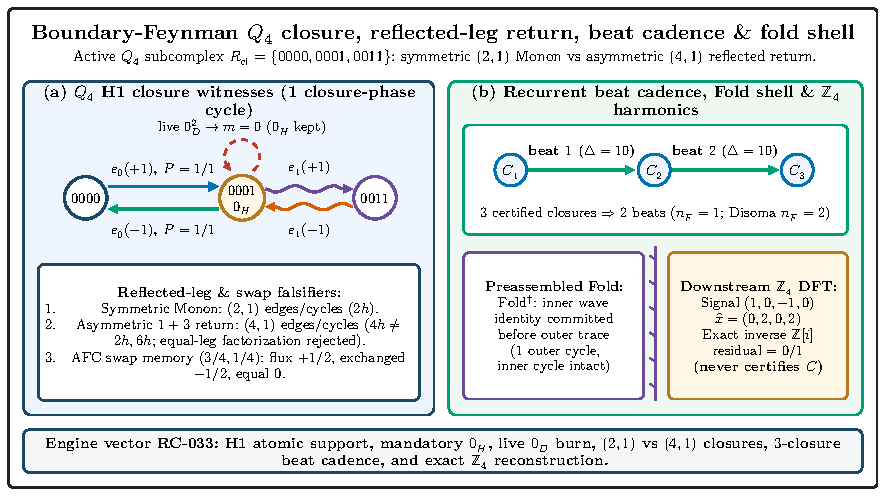
\includegraphics[width=0.92\linewidth,height=0.78\textheight,keepaspectratio]{figures/generated/native-closure-q4-dec-walk.pdf}
\caption{Boundary-Feynman $Q_4$ closure, asymmetric $(4,1)$ return, three-closure beat cadence, preassembled $\operatorname{Fold}^{\uparrow}$ shell, and downstream $\mathbb{Z}_4$ harmonic readout (\texttt{native\_closure\_wave\_dec\_walk.csv}).}
\label{fig:manual-native-closure-q4-walk}
\end{figure}

\begin{table}[H]
\centering
\caption{Eight-stage $Q_4$ D.E.C. closure, beat, fold, and $\mathbb{Z}_4$ harmonic ledger (\texttt{RC-033}).}
\label{tab:manual-native-closure-dec-walk}
{\footnotesize
\begin{tabular}{llllrrl}
\toprule
Stage & Scope $B$ & $v\to v_e$ & Slot / role & $w$ & $P(e;B)$ & D.E.C. audit outcome \\
\midrule
\texttt{M1\_leg\_out} & $B_{\mathrm{monon}}$ & $0000\to0001$ & $e_0(+1)$ & 1 & $1/1$ & H1 branch out \\
\texttt{M1\_hinge\_dwell} & $B_{\mathrm{monon}}$ & $0001\to0001$ & $0_H+0_D^2$ & 1 & $1/1$ & $0_H$ kept; $0_D^2$ burned ($m=0$) \\
\texttt{M1\_return\_cert} & $B_{\mathrm{monon}}$ & $0001\to0000$ & $e_0(-1)$ & 1 & $1/1$ & certified return: $(2,1)$ edges/cycle \\
\texttt{M2\_asym\_4step} & $B_{\mathrm{asym}}$ & $0000\leftrightarrow0011$ & $e_0,e_1(\pm1)$ & 1 & $1/1$ & reflected $1+3$: $(4,1)$ edges/cycle \\
\texttt{M3\_beat\_cadence} & $B_{\mathrm{wave}}$ & $0000\leftrightarrow0000$ & $\operatorname{bip}_1\dots3$ & 3 & $1/1$ & cuts $(0,10,20)$: $2$ beats, $n_F=1$ \\
\texttt{M4\_fold\_expose} & $B_{\mathrm{fold}}$ & $0000\to0100$ & $\operatorname{Fold}^{\uparrow}(+1)$ & 1 & $1/1$ & $1$ outer cycle; inner wave intact \\
\texttt{M5\_afc\_swap} & $B_{\mathrm{swap}}$ & $0000\to0001$ & $e_0(+1)$ & 3 & $3/4$ & AFC flux $+1/2$, swapped $-1/2$ \\
\texttt{M6\_z4\_harmonic} & $B_{\mathrm{harm}}$ & $0000\to0000$ & $\mathbb{Z}_4$ DFT & 4 & $1/1$ & $\hat{x}=(0,2,0,2)$, recon residual $0/1$ \\
\bottomrule
\end{tabular}
}
\end{table}
